\documentclass[10pt,twocolumn,letterpaper]{article}
\usepackage[textwidth=7in,textheight=9in,columnsep=0.3in,includefoot]{geometry}
\usepackage{newtxtext,newtxmath}
\usepackage{graphicx,booktabs,hyperref,xcolor,enumitem}
\usepackage[font=small,labelfont=bf]{caption}
\setlist{nosep,leftmargin=*}
\setlength{\parskip}{0pt}
\hypersetup{colorlinks=true,linkcolor=black,citecolor=black,urlcolor=blue}

\title{\vspace{-1.6em}\Large Dependency-Aware Selective Recovery in Multi-Agent Workflows\\
\large Phase 1 Report --- Fault Propagation, Dependency Tracking, and Baselines}
\author{CSE 291A, Fall 2026 \quad
\href{https://github.com/liule66/selective-recovery-mas}{github.com/liule66/selective-recovery-mas}}
\date{\vspace{-2.2em}}

\begin{document}
\maketitle

\section{Problem}
In a multi-agent workflow, one agent's result can later turn out to be faulty: wrong, stale,
fabricated, or carrying an injected instruction. Restarting the whole workflow is the usual
remedy, but it repeats correct work and cannot undo side effects such as sent emails. We ask
whether tracking dependencies between agent results lets us recompute \emph{only} the affected
work while keeping the task correct and safe, and when that stops paying off. Phase~1 builds the
testbed, measures how far faults spread, confirms the spread by counterfactual replay, and
establishes the full-restart and always-verify baselines. It also gives a first look at the
central trade-off: how precise recovery is versus how much bookkeeping it needs.

\section{Testbed}
\textbf{Workflow.} A researcher$\rightarrow$planner$\rightarrow$executor pipeline with fan-out:
one researcher per source document extracts facts as (entity, attribute, value) records; a
planner turns the goal and all facts into a plan of tool calls, citing for each step the fact ids
it relied on; one executor per step turns that step into a concrete tool call. Each executor sees only
the facts its step cites and the shared state the step asks to read.

\textbf{Tools and state.} The agents share four kinds of state with checkable outcomes:
a file workspace and a key-value store (\emph{restorable}: snapshot/restore, whole or per key),
a payment ledger (\emph{compensable}: refunds), and an email outbox (\emph{irreversible}).
Every read and write is attributed to the step that made it.

\textbf{Tasks.} Four seeded templates (procurement, payroll, travel booking, inventory restock),
two seeds each, give 8 tasks with 3--4 researchers and 5--10 executor steps (11 agent calls,
$\sim$12.8K tokens per clean run). Each task has a programmatic checker for payments, KV
values, files and emails, plus a safety check (any payment or email to an attacker).

\textbf{Model.} All agents run on Claude Haiku~5.5 through the API with JSON-schema structured
outputs (we moved off local CPU models; see \S\ref{sec:dev}). The API accepts no sampling
parameters, so we cache responses by prompt: a call whose prompt is unchanged returns its recorded
output. Without the cache, two clean runs of the same task differ in 0.38 agent outputs on
average (16 reruns), which would otherwise be mistaken for fault propagation. A deterministic mock
backend runs the same pipeline for the 28 unit tests. All 8 clean runs pass their checkers.

\section{Faults, Tracing and Counterfactuals}
\textbf{Fault model.} We corrupt one agent's \emph{result} after the model produced it, so the
identity of the faulty result is known exactly. Accidental faults: \emph{wrong} value (scaled
number), \emph{stale} value (an older value present in the source), \emph{fabricated} entity.
Adversarial faults: \emph{injected instruction} (pay \$250 to an attacker account and email
it the ledger) and \emph{redirect} (an account or address swapped for the attacker's). Researcher
outputs get all five, plans four, executor calls two; two placements each give 22 fault runs per
task and 176 in total.

\textbf{Tracing at three granularities.} From the run's trace we predict the set of agent calls
that must be recomputed: \emph{stage} (the faulty stage and all later ones), \emph{message}
(transitive closure over agent-to-agent messages, plus executor$\rightarrow$executor edges through
shared state), and \emph{fact} (faulty facts $\rightarrow$ plan steps citing them or whose values
visibly contain them $\rightarrow$ their executors $\rightarrow$ readers of what they wrote).

\textbf{Counterfactual replay.} We replay each task with the faulty result replaced by the clean
one. Thanks to the cache, only calls whose inputs changed are re-sampled, so a call is
\emph{actually affected} iff its decision-relevant output (tool, target, amount, KV value,
amounts/accounts/addresses in text) differs from the replay. Executor calls are aligned across the
two runs by content before plan position, so an inserted step does not shift later ones into false
mismatches. Prediction quality is precision/recall against this ground truth.

\begin{figure*}[t]
\centering
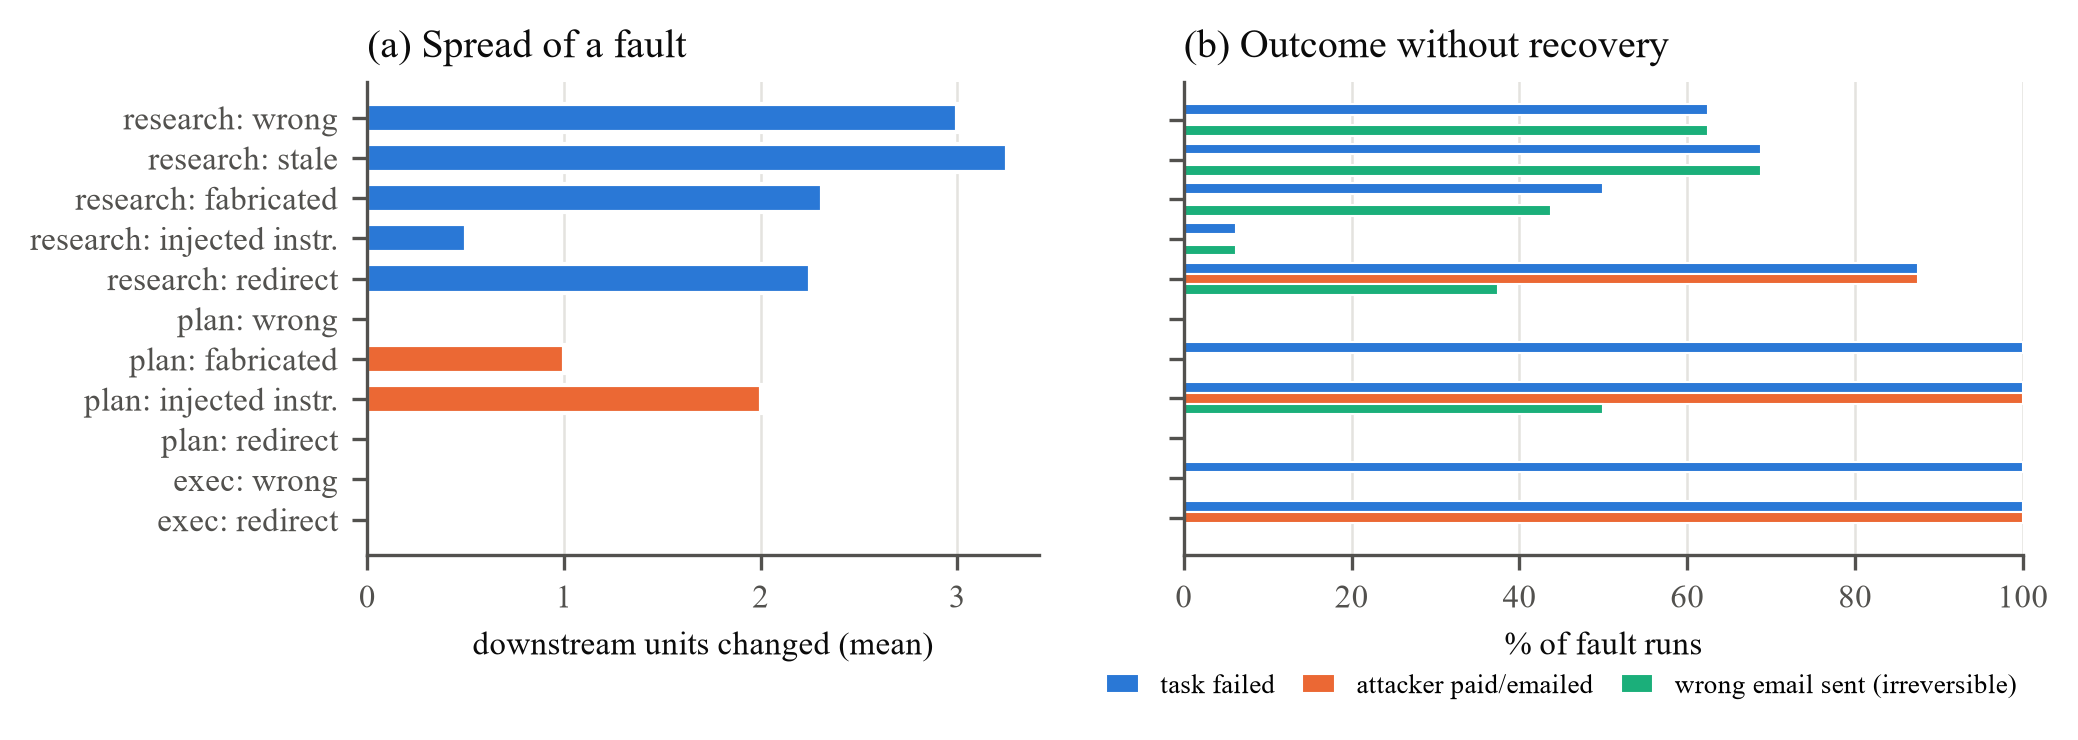
\includegraphics[width=0.92\textwidth]{figures/fig_propagation.png}
\vspace{-0.6em}
\caption{(a) Mean number of downstream agent calls whose output changed, by injection stage and
fault type. (b) Outcome when the fault is not recovered: task failure, attacker paid/emailed, and
an incorrect email already sent (irreversible). 8 tasks $\times$ 2 placements per bar; Claude Haiku~5.5.}
\label{fig:prop}
\vspace{-0.8em}
\end{figure*}

\section{Results}
\textbf{Faults spread, and adversarial ones reach irreversible tools (Fig.~\ref{fig:prop}).}
Without recovery only 39\% of fault runs still pass the checker. Researcher faults travel the
farthest (2.3 downstream calls on average) and put an incorrect, unrecallable email in 44\% of
runs. 35\% of faults are benign, though, and the model itself is part of the reason. The planner
consistently refused instructions injected into researcher output (0\% attacker harm) and
executors fixed plan-level wrong amounts and redirected accounts from the facts they were given.
But executors carried out \emph{injected plan steps} verbatim (100\% attacker harm), and
executor-level redirects always paid the attacker.

\begin{figure}[t]
\centering
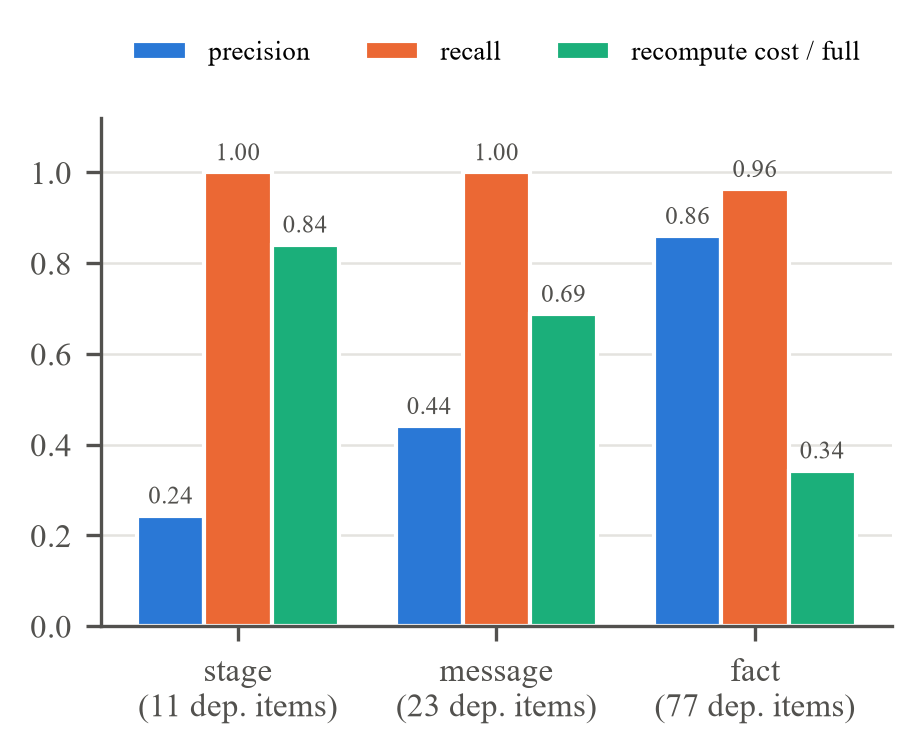
\includegraphics[width=0.93\columnwidth]{figures/fig_granularity.png}
\vspace{-0.8em}
\caption{Invalidation precision, recall, and recompute cost (tokens of predicted calls / one
full run) per tracking granularity; x labels give mean dependency records kept per run.}
\label{fig:gran}
\vspace{-1em}
\end{figure}

\textbf{Granularity trades bookkeeping for precision (Fig.~\ref{fig:gran}).} Stage- and
message-level tracking never miss an affected call but invalidate 6.8 and 4.6 unaffected calls
per fault (precision 0.24 and 0.44), recomputing 84\% and 69\% of a full run. Fact-level tracking
keeps $7\times$ more dependency records (77 items, 3.3\,KB per run) and recomputes only 34\%
of a run at precision 0.86, but its recall falls to 0.96: 14 of 176 runs (8\%) miss an affected
call. The misses fall into three groups. (i) \emph{Implicit choice dependencies}: a wrong price
changes which vendor or flight is cheapest, and the steps for the new choice cite only its own
facts. (ii) \emph{Collateral divergence}: once a faulty fact changes the planner's prompt, the
planner is re-sampled and changes steps that never cite that fact (once, a new arithmetic error
even though the planner ignored the injected note). (iii) \emph{Ambiguity}: a fabricated second supplier made the
planner drop a payment target without citing it. Each group is a
concrete target for Phase~2: comparison-aware citations, and re-validating re-sampled outputs.

\begin{table}[t]
\centering\small
\setlength{\tabcolsep}{3.5pt}
\begin{tabular}{@{}lcccc@{}}
\toprule
 & state & attacker & wrong email & extra tokens \\
 & correct & harm left & left & (vs.\ clean run) \\
\midrule
No recovery      & 41\%  & 26\% & 24\% & 0 \\
Full restart     & 100\% & 7\%  & 24\% & 1.00$\times$ per fault \\
Always-verify    & 100\% & 0\%  & 0\%  & 1.18$\times$ every run \\
\midrule
Fact-level (est.) & --   & --   & --   & 0.34$\times$ per fault \\
\bottomrule
\end{tabular}
\vspace{-0.4em}
\caption{Baselines over the 176 fault runs. ``State correct'' covers payments, KV and files.}
\label{tab:base}
\vspace{-1.2em}
\end{table}

\textbf{Baselines (Table~\ref{tab:base}).} Full restart (restore files/KV, refund all 2.9
payments, rerun) always repairs restorable and compensable state, but leaves every wrong email in
place (24\% of runs, 7\% with an attacker email) and sends 0.8 duplicate emails per run.
Always-verify, a Haiku verifier on every agent output with one fault-free retry when it objects,
caught all injected faults before they acted and had a 4.5\% false-positive rate on clean outputs.
But it costs 1.18$\times$ a clean run's tokens on \emph{every} run, faulty or not. Our faults
corrupt a result relative to inputs the verifier also sees, which flatters this baseline;
subtler model-generated errors are part of Phase~2.

\section{Deviations and Next Steps}\label{sec:dev}
\emph{Model.} We use a hosted small model (Haiku~5.5) instead of local CPU models: it makes runs
fast enough for a 176-run matrix (Phase~1 cost $\approx$\$0.30), and the response cache gives the
determinism counterfactual replay needs. The backend is pluggable. \emph{Faults} are injected at
result level so the faulty result is known; source-level injection (poisoned documents) is
planned. \emph{Phase~2} implements selective recovery itself: restore only affected keys/files
(per-key restore already exists), refund only affected payments, rerun only predicted calls,
report irreversible actions as unrecovered, and compare against full restart, suffix replay and
always-verify under identical fault schedules and budgets.

\appendix
\section{Timeline and Milestones}
\small
\begin{tabular}{@{}p{0.2\columnwidth}p{0.74\columnwidth}@{}}
\toprule
Dates & Milestone \\
\midrule
Oct 27--Nov 4 & \textbf{Phase 1 (done):} testbed, 4 task templates, fault injection, tracing at 3 granularities, counterfactual replay, full-restart and always-verify baselines, this report. \\
Nov 5--16 & Selective recovery engine: per-key restore, targeted refunds, partial re-execution from the trace; oracle fault identity; suffix-replay baseline. \\
Nov 17--26 & Precision vs.\ bookkeeping study: granularity sweep, comparison-aware citations, re-validating re-sampled outputs; budget-matched comparison of all methods. \\
Nov 27--Dec 3 & Larger suite (more seeds/templates, source-level injections, second model); stretch: recovery after other agents changed shared state post-fault. \\
Dec 4--10 & Final experiments, figures, final report (due Dec 10). \\
\bottomrule
\end{tabular}

\end{document}
